\documentclass[11pt]{labbook}
\usepackage[utf8]{inputenc}
\usepackage{graphicx}
\usepackage[margin=1.0in]{geometry}
\usepackage{outlines}
\usepackage{enumitem}
\usepackage{setspace}
\usepackage{listings}
\usepackage{color}
\usepackage{array}
\usepackage{amsmath}
\usepackage{float}
\usepackage{verbatim}
\usepackage[final]{pdfpages}
\usepackage{caption}
\usepackage{subcaption}
%%%%%%%%%%%%%%% Section for new commands %%%%%%%%%%%%%%%%%%%
\newcommand{\Loss}[2]{L\left(#1,#2\right)}

%%%%%%%%%%%%%%% End %%%%%%%%%%%%%%%%%%%%%%%%%%%%%%%%%%%%%%%%
\setenumerate[1]{label=\Roman*.}
\setenumerate[2]{label=\Alph*.}
\setenumerate[3]{label=\roman*.}
\setenumerate[4]{label=\alph*.}
\title{Lab Notebook}
\author{Alex Cope}
\date{August 2016}

\begin{document}
\maketitle
\tableofcontents



\labday{GST Preliminary exam notes}
\experiment{Topic: Protein Evolution}
\subexperiment{Review on integrated view of protein evolution by Pal et. al \cite{pal2006review}}
One of the strongest predictors of protein evolution rate is expression level. The higher the expression level, the slower the rate of evolution, which is sometime referred to the E-R anticorrelation. The importance of the protein (its dispensability) is a relatively poor predictor. 
Many amino acid chages due to positive selection (contrast to expectations from neutral theory)

\subexperiment{Review on determinants of rate of protein sequence evolution by Zhang and Yang \cite{zhang2015review}}
Questions left to be answered:
\begin{enumerate}
\item Expression cost hypothesis of the E-R anticorrlation lacks definitive empirical evidence and main components of expression cost have not been specified
\item Interdependency, relative contributions, adn combined explanatory power of multiple identified causes of E-R anticorrelation are unclear. Additionaly, what other causes exist?
\item Apart from mistranslation, protein misfolding and misinteraction, other cellular and molecular errors, such as transcriptional error, splicing error, RNA editng error, translation initiation from upstream start codons and translational stop codon readthrough, have not been investigated for potential effects on protein evolutionary rate
\item Distribution of fitness effects of mutations in a gene plays an important part in determining the rate of protein sequence evolution, but details have not been elucidated empirically, although work by Stiffler et. al. (Cell 2015) and Podgornaia et. al. (Science 2015) are examples of progress. Functional basis of fitness distribution is more difficult to identify.
\item Cellular errors may by chance create new protein variants, it would be interesting to study whether these errors have important roles in the origin of new protein functions and adaptation
\item Mechanisms underlying correlations between protein evolutionary rate and factors discussed in this review are unknown, requires integrative approach to understand interdependencies between factors (see review for references)
\item How do these factors apply to noncoding RNAs
\item Evolutionary rate of protein can change during course of evolution, but factors underlying these changes remain unknown
\item Connecting differences of rates between proteins to differences in rates between protein regions. See references in reviews.
\end{enumerate}



\labday{Progress Tracker}
\experiment{8-25-2016}
\subexperiment{Reading}
1. Li \textit{et al}.
Whole genome analysis of non-optimal codon usage in secretory signal sequences of \textit{Streptoyces coelicolor}. \textit{Biosystems}. 2006
\newline
2. Zalucki \textit{et al}. Secretory signal sequence non-optimal codons are required for expression and export of b-lactamase. \textit{Biochemical and Biophysical Research Communications}. 2007
\newline
3. Read Chapter 2 out of Lynch 2007.
\let\cleardoublepage\clearpage

At Cedric's recommendation, I re-ran the \textit{E. coli} simulations with more samples (10,000 up to 50,000). He pointed out that the frequency plots for the codon usage were a little flat, which would be reflected in the traces not converging. The traces looked okay, but I decided it wouldn't hurt to rerun them with a few more samples. The plots looked almost identical, so it seems like 10,000 samples is sufficient for the \textit{E. coli} genome. One of the peptides that looks particularly flat is for Lysine (K). The AAA codons is favored at a frequency of ~0.8, regardless of log$\phi$. In \textit{E. coli}, AAA is the best initiator of translation. I wonder if this plays a role in the strong bias for AAA.
\newline
Also ran for \textit{C. bescii} and received the data on \textit{E. coli} gene expression from the Li 2014 paper.
\newline
Mallory Ladd (in Bob's lab) asked me to write some scripts from her for a project she is working on last week. She reminded me on today, so I decided to finish that up. Most of the scripts were based on work I did during my rotation in Bob's lab, but her files were in a different format. This required me to make modifications to my previous scripts, which turned out to be more annoying than I thought it would be.

\experiment{8-26-2016}
Finished up the scripts for Mallory and ran them for her. When I have a chance during the weekend, I will spend time learning how to use LaTeX, grading the short essays I assigned my students on the role of computation in unlocking biological systems, and finish preparing for lab on Monday.


Also, touched base with Steve regarding the protein clustering project he and I worked on during my rotation. He is collaborating on a similar project with Dr. Barerra over in BCMB and said he is planning on giving the project to an undergrad. After the undergrad has done some initial calculations, he said I'm welcome to help out on creating some "relatively low hanging" simulation code. Depending on how work is progressing with my other projects, I would like to help out on this where I can. 

\subexperiment{Goals for next week}
1. Compare gene expression results from ROC simulations with results from Li 2014.

2. Look at gene expression results for the genes with predicted signal peptides. See if the majority of them are low expression genes (ie. non-optimal codon usage could be largely due to mutation biases).

3. Begin thinking about how to handle house-keeping genes in current models.

4. Resume independent-study of Bayesian Data Analysis.


\experiment{8-29-2016}
Next steps for analysis:\newline
1) Fit model to genome consisting of genes with the first 35 amino acids removed, which should eliminate most of the signal peptide components. I would expect that if signal peptides have evolved under different selective pressures, then the overall model fitting would improve. However, given the large size of most genes relative to the signal peptides, I don't know how much impact removing these will have even if the signal peptide region and the rest of the gene are evolving differently. 

2) Fit model to just genes with predicted signal peptides and do a separate model fitting to genes without predicted signal peptides. If genes with signal peptides are evolving differently, I would expect to see a drop off in the fitting relative to the genes without signal peptides. The number of genes with predicted signal peptides is roughly 10 percent of the E. coli genome (425 genes), so I don't know if this will be enough to get accurate fittings. Maybe I could create a random subset of 425 genes without signal peptides and fit the model to this subset in order to eliminate size as a variable in the analysis.

3) I would like to perform analysis with the mixture models that we discussed yesterday. It makes sense to me to treat genes with signal peptides vs those without as separate subpopulations within the genomes. I'm also wondering if it would be possible to go a level deeper in this analysis and treat individual codons as a member of a signal peptide vs a non-signal peptide. To me, this seems like a more accurate approach since it is the regions within the gene that could be evolving differently. However, my understanding of mixture models is limited and my knowledge of the current implementation in ROC even less so. Currently reading Gelman's chapter on Finite Mixture Models in order to improve my understanding. 

\experiment{8-30-2016}
Submitted the above to Mike here are his responses.

1) Only one way to find out.  Key question is how will you compare the quality of the model fits? 

Me: Read up on model checking in Gelman's book

2) Creating a 'control' set makes sense, but note that the quality of the fit is quantitatively described by the  posterior parameter intervals (more info, tighter intervals) and measures of model fit based on the unscaled probabilities of the MCMC samples.

3) For the first part, I would agree this would be a good step. If you use the mixture model approach, you can initially designate genes into particular category and let the algorithm update these designations.  Preliminary work 
suggests that using estimates of $\phi$'s when fitting the model helps with the categorization.

Me: Have this from Li et al (2014, Cell). 

For the second part, I agree that trying to apply separate models to different parts of the gene would be nice.  How to do this in the current framework will take some thought.  Note that I am interested in a similar type of analysis at the level of separate introns for alternatively spliced 
genes. 

Completed a run of the truncated genome, but a problem occurred when trying to plot these functions. Mike suggested I look into writing the objects to a file. Looked into the parameterObject.r class and found a writeParameterObject function, which seems to accomplish this task. Added it to my standard template script for running ROC. Now if something happens when plotting or I want to go back to do more analysis on a run, this object will be saved to a file. 

Mike noted that I need to understand where the sources of the data come from. Li et al (2014, Cell) performs their subexperiments using ribosome footprinting. The mRNA levels they provide are RPKM values, which are normalized by the length of the gene. 


\experiment{8-31-2016}
Towards the end of the day, got the following error while attempting to fit ROC to a genome consisting of only genes containing signal peptides. When the the function to plot the CUB plot was called, I got a memory allocation issue with the following traceback:


I ran this on Gauley with the most up-to-date version of the RibModel. I moved this file over to my computer with a slightly old version and did not get this error. I sent Holis all the information I could in hopes that he could figure out what is going on.

\experiment{9-1-2016}

Since I've been wanting to get into the code a little more, I figured trying to debug this myself wouldn't be a bad idea. Based on what I found, it seems like the writeParameterObject() function in R is intended to create a Parameter object that will be used \textbf{just} for future data analysis, not a starting point for a new run. Maybe that is what was intended, but I think this is bad software practice. If you have two objects of the same class, then they should work the same way.

The place where things are breaking is at the call for ROCModel::updateTracesWithInitialValues(Genome \&genome). The source of this error seems to be that many of the variables that are needed for fitting a model are initialized in the initParameterSet() function. This function is only called from the constructors of the Parameter subclasses; as a result, they will only be initialized when the initializeParameterObject() is called in R. 

The loaded Parameter object does not see groupList, which is an array containing the amino acid letter ids (ie. K for lysine). This can be fixed by moving the initialization of this list to the Parameter.h file. I still need to do some digging into this.

\experiment{9-2-2016}
I continued some of the debugging from yesterday. I also was unfortunate enough to encounter the error from August 31st again on my local machine. However, I have not had much luck consistently generating this error, so what the cause of it is baffling me. 

However, I did find a fairly significant error in  Genome::getGenomeForGeneIndicesR(), which returns a genome consisting of the genes in a mixture. In the plotModelObject.R (generates CUB plots), it looks like it pulls out the genes in a mixture and passes into Genome::getGenomeForGeneIndicesR() a list of the indices for these genes. The problem is these indices are based on an R vector (starts at 1), but the code in Genome::getGenomeForGeneIndicesR() forgets to subtract off 1 to convert the indices to C++ array indices (starting at 0). In the case of a mixture model with only 1 category, this just means the genome returned will be missing the fist gene and contain a blank gene in the last position in the gene array. However, when fitting using mixture categories, this means you could be missing a lot of genes. I'm not surprised this error was not found sooner because of C/C++ not returning an IndexOutOfBounds error when accessing array/vector elements via array[index]. It is generally safer when working with std::vector<> to use vector.at(index), as this will return an IndexOutOfBounds error. However, it is also slower. 

I talked with Bob before I called it a day. I explained to him some of the problems with previous analysis of codon usage bias for signal peptides in \textit{E. coli} (ie. failure to account for affects of varying gene expression) and showed him some of the plots I generated. I also explained to him the next steps I want to take with the analysis. He said he was happy about what I have done so far and where I plan on going with this project.

\subexperiment{Plans for Weekend}
Continue reading "Part 2: Fundamentals of Bayesian Data Analysis" from \textit{Bayesian Data Analysis}, 3rd ed, Gelman et al and "Chapter 7: Model Assessment and Selection" from \textit{The Elements of Statistical Learning: Data Mining, Inference, and Prediction}, 2nd ed, Hastie et al.

Also review the chapter on numerical integration from \textit{Numerical Methods}, 4th ed, Faires and Burden. This thing about dividing a Gamma distribution up into quantiles and taking the average value of each just seems wrong to me. 

\experiment{9-6-2016}
Focused on learning about model checking. I just want to get a solid base in this area by the end of this week so I can start implementing some model checks. So far, looking like the Bayesian Information Criterion (BIC) might be a good start, but I want to read up on it a little bit more. I know Gelman et al talks about it and Hastie et al cite the original paper, which also might be worth taking a look at. 

Last week, Mike noted that sometimes it is hard to tell if the traces are actually converging based on the plots. I think adding a moving average function might make this task a little bit easier. 

In one of the earlier SignalP paper, the authors note that SignalP should not be used to identify extracellular proteins; instead, researchers should use SecretomeP (by the same group). This brings up a good point: most of the papers that have done analysis of codon usage bias in signal peptides have seemed to imply that signal peptide = extracellular. It might be worth dividing up those with signal peptides into two groups: those that are predicted to be extracellular via SecretomeP and those that are not and fit these in ROC with a mixture model. 

\experiment{9-7-2016}
Talk to Cedric about autocorrelation functions. Look at Geweke scores. 


\experiment{9-11-2016}
Since 9-7-2016:
$\bullet$ Set up a Github repository for Bob's lab. Should make it easier for us to keep track of the scripts we write and make accessing them easier. I also commented/documented some of the scripts I had previously written to make them more accessible to my labmates who have little programming experience. \newline
$\bullet$ Got a little bit of experience working with the Python package, Pandas. Supposed to be good for data analysis, which is why Yaojin has suggested teaching it in LFSC 507. \newline
$\bullet$ Looked into autocorrelation functions and MCMC checking methods, including the Geweke score. \newline
$\bullet$ Performed an autocorrelation on the $\Delta\eta$ and $\delta$M traces using R's acf function. Generally, they looked something like this.

\fbox{\includegraphics[page=8,scale=0.5]{Model_checking/Autocorrelation_just_genes_w_sigpep.pdf}}

$\bullet$ I also ran the acf for the loglikelihood trace and obtained results that generally looked like the following.
\newline
\fbox{\includegraphics[page=1,scale =0.5]{Model_checking/acf_loglikelihood.pdf}}
\newline
$\bullet$ Started NSF Graduate Fellowship application.

\experiment{11-17-2016}

\subexperiment{Summary of work since last update}
October was mainly driven by NSF GRFP application, colloquium presentation for Grant Writing, and writing NSF-style proposal for Grant Writing class. Time dedicated to TAing for the LFSC 507 class has not been insignificant as I had to learn the Python packages NumPy, SciPy, and Pandas for some of my lectures. 
\newline
However, I was able to make significant progress on the Signal Peptide project (see section "Signal Peptide Project - Progress as of 11-17-2016" for details).
\newline \newline
Mike's comments regarding current results: \newline
$\bullet$ Overall, it seems like selection on CUB within signal peptide regions is in the same direction as the rest of the genome. However, there might be some differences in the strength of selection for certain codons. \newline \newline
$\bullet$ Standard linear regressions were used for generating the plots found in the Signal Peptide Project section. Weighted least squares regression would be a more valid approach due to the deterministic variables in these cases are not equally precise. I can modify the function I used to generate these plots to take in a boolean variable specifying whether or not the user wants to use ordinary or weighted least squares and perform the appropriate calculations. (Note: need to look into weighted least squares first). \newline \newline
$\bullet$ When treating $\Phi$ values as given and not estimating them, treated them as the true $\Phi$ value, ie. variation in $\Phi$ is 0. This is certainly not the case. A better approach might be to calculate the average standard deviation for each $\Phi$ from the different samples and use these to allow the genes to vary when estimating $\Delta\eta$. I will need to measure the autocorrelation of the $\Phi$ traces to make sure the samples are independent of the previous samples. \newline \newline
$\bullet$ Results for the signal peptides and first 31 codons in genes lacking a signal peptide (Figures 5a and 7a) seem more consistent with selection against nonsense errors in the 5' regions of the genes. To be more certain of this, instead of doing first 31 codons for all genes, can calculate mean and variance of signal peptide length and use these to draw cutoff points for splitting the genes. Signal peptide regions are generally 20 to 40 amino acids long. An alternative approach is take the first 20 codons,truncate out the next 20, and then take the the rest of the gene. \newline \newline
$\bullet$ Would be helpful if plots comparing $\Delta\eta$ values between mixtures generated by module plotParameterObject.R also included error bars. \newline \newline

Other current work:\newline
1) The plotModelObject.R module cannot generate the codon usage frequency plots (as function of $log\Phi$) when not estimating expression. I started fixing this on 11-16-2016. Part of the problem with the current implementation is it relies on making calculations from the last samples of the traces. When not estimating a parameter, the traces for that parameter are not updated, resulting in the traces being filled with the value 0. I'm modifying the code to initialize the $\Phi$ traces with the initial values provided by the user. If no values are provided, the traces will be initialized with 0.0, as they are now. The advantage of this is it allows us to handle this situation of not estimating parameters without requiring a bunch of if-else statements to the code.
\newline
2) In Bob's lab, I promised to assist Mallory Ladd with the data analysis for a project she is currently working on and will present at a conference in a few weeks (with the promise of being listed as a co-author on the project). This project involves looking at liquid chromatography tandem mass spectrometry (LC-MS/MS) measurements of metabolites in soil water samples. Metabolomics data is usually more complicated than proteomics data because of the greater variability in the chemical structures of metabolites relative to peptides. 
\newline
3) I need to finish modifying the current ribModel framework to treat $\Phi$ as a mixture of lognormal distributions. I need to implement the traces to keep track of the additional hyperparameters approximated by the model and actually test the code to make sure it works. \newline \newline

Other stuff: \newline
$\bullet$ Assisting older students in GST with their preliminary exam by providing feedback on proposals/presentations. This has given me some insight into the GST prelim process. The combination of this and Grant Writing should result in my own prelim going smoothly next year...hopefully. \newline
$\bullet$ Signed up for Outreach on Darwin Day website. I suggested last night at the meeting for Darwin Day that we consider doing something similar to "Pint of Science" which will allow general public to interact with scientists in a more informal context. I already harassed a couple of my closer friends in GST and they seem interested in helping out.
$\bullet$ Final draft of proposal for Grant Writing is due November 22nd by 5 pm, so I've been working on making some edits to that the past couple of days.
\newline
Plans for the coming month (ordered by my current priority):
1) Make improvements to statistical approach and plots based on Mike's suggestions. Bob has said he would also like me to look at signal peptides in \textit{C. thermocellum} and \textit{C. bescii}, but I expect we will find similar results to \textit{E. coli}. Given the relatively short time it takes to fit ROC to data, it wouldn't hurt to perform the additional runs.   
2) Assist Mallory with data analysis. Poster presentation is in a few weeks. We have exchanged a few papers regarding metabolomics and current data analysis tools. We are meeting tomorrow (11-18-2016) to discuss ideas.
3) Finally finish $\Phi$ mixture distribution. 


\experiment{11-18-2016}

\subexperiment{Meeting with Mallory}

Meeting to discuss analyzing data from LC-MS/MS runs on soil water data.

First step is defining metabolite features based on mass and retention time, but these are dependent on sample preparation and data acquisition (so like a hierarchical model). Choice of solvent, biological matrix, etc. can affect factors such as elution and chromatographic separation. Artifacts can be generated based on desorption and ionization processes. In summary, results are highly dependent on experimental parameters and sample preparation. [Yao \textit{et al}, Metabolites, 2015]
\newline

Mallory has a bunch of samples. Each file contains MS1 and MS2 scan info for top 10 most abundant in each MS1 scan. 

\experiment{12-7-2016}
Have been looking into linear errors in variable models. Have not been able to find much that makes immediate sense to me. However, there are two potential programs/packages I might be able to take advantage of. Leiv is a R package that came out a few years ago. Seems to take Bayesian approach. STATA also has some tools. UTK students have access to STATA through 


\subexperiment{Gilchrist lab meeting}
Phi is expression rate observed given current set of amino acids and psi is the expression at the optimal amino acids. Adjusted gene expression is psi/phi. So if you have psi of 1 and phi of 0.8, need to produce 20 percent more.

Read McCandlish papers Mike sent today.

E-score in BLAST means the likelihood of finding a match just by chance, the lower the better. 

Description of ROC paper...possibly help Cedric with paper and documentation

Get on the gene expression mixtures.  

Would probably be a good idea to take some more formal statistics classes in the next few years. I emailed Russ to ask if he knew any good courses to take. He recommended:

Math 525 and 526 or Stat 563 and 564. These are both series courses to be taken over the course of one academic year. He also recommended Stat 577, Data Mining. 

Added confidence intervals to module for plotting Parameter objects in RibModelFramework. Also have altered code to work make CUB plots even when not estimating expression. This fix was implemented by initializing traces with initial values if present. I want to test this a little bit more before I push anything to the repository. 

\experiment{12-8-2016}
Working on finishing up the mixtures of gene expression values. Found a typo in the code that caused R to not be able to see some of the functions for getting the $s_\phi$ trace. Code currently compiles and runs. 

Bob and I discussed last week about redoing the analysis for signal peptides only using genes predicted to have a signal peptide with a high D-score (>0.75). The D-score is a weighted average of other metrics approximated by SignalP. From my understanding, the closer the score is to 1.0, the better the prediction. My understanding of the details will require me to read the SignalP papers (probably for both versions 3.0 and 4.0). For \textit{E. coli}, there are 266 genes that fall into this category. 

Read up on some linear regression stuff. Signed up for some Coursera lectures on regression modeling, statistical inference, and genetics/evolutionary biology. My guess is these are geared more towards undergraduate, but they might have some information useful to me. I can have the lectures playing in the background while I work and if something should sound unfamiliar, I can pause my work to pay closer attention. Also read a little bit from \textit{The Elements of Statistical Learning}.

\experiment{12-12-2016}
Having issues implmenting gene expression mixture. Currently getting a segmentation fault. 


\experiment{12-14-2016}
\subexperiment{Gilchrist Lab Meeting}
SMA R package -> look into

HMM make inferences about shifts in optimal amino acids

Cedric will be taking over plotting $\phi$'s to Selac for empirical.

Meeting with Albrecht's lab at 3 pm. 

Make people do commits and pushes more often to GitHub

Github book that is free online. Software Carpentry might be worth looking into, also.

\subexperiment{Meeting with Albrecht and Ricardo}
Group from UK, mRNA levels in yeast, 600 transcripts oscillate over cell cycle fine resolution time. Use graph algorithm for studying biological networks

Thermodynamic analysis -> use chemistry concept to analyze networks
	- Entropy and information
	- Difficult to tell things from current analyses
	- We're interested because cyclical data, can methods be applied to 			  circadian rhythms
	 

Data collected is very descriptive in nature. Growth rate, meristems of root, translation regulation of genes involved in control of cell cycle. Periodic. Generate ribosome footprint data. Ribosome TRAP genetically label ribosome in certain cell types, pull down specific ribosomes from certain types. Express genetically modified ribosome proteins under certain tissue specific conditions.  

Albrecht has talked to the Pakanara's group about teasing out networks of translational efficiency (function of ribosomes per mRNA). Plenty of published data sets. Have not been analyzed comprehensively. 

Big questions:
1) When plants are exposed to two different conditions, some genes will be expressed similarly, some will be different. What does this tell us about signal transduction? Different conditions sometimes results in similar expression patterns. Why? 

Lack time series data at translation level, but might have it at transcriptional level. 

Signal transduction -> apply different stressors, do these affect different genes in the same way or not. One particular group (ribosomal proteins) of mRNAs respond to a wide-range of conditions can be target. These proteins are highly regulated at translation level. Ribosomal proteins appear to be co-regulated. If you look closely, you can convince yourself that these are actually different. Is this true? 

Mike proposes we think about current framework Ricardo is working with, and modify it to work with this project. Ratio of $\kappa$ to $\delta$. Tease out differeces between $\kappa$ and $\tau$. 


\experiment{12-15-2016}

Git tutorial:
1) Create new directory and while in the directory use git init command
2) Use git add <filename> to track changes to file(s)
3) Can use git status to check for changes
4) Can commit using git commit -m "<message>"
5) Can add remote repository with git remote add <remote name> <repository url>
6) Push to remote repository with git push -u <remote name> <branch name>. 
-u tells git to remember these parameters for later use, can just enter git push
7) git pull <remote name> <branch> to get changes from remote repository
8) git branch <branch name> to create a new branch
9) git checkout <branch name> to look at a new branch 
10) git merge <branch> to merge changes made in branch with current branch
11) can unstage a file using git reset <file name>
12) git checkout -- <file name> can be used to go back to last commit

\subexperiment{Student comments regarding LFSC 507}
$\bullet$ Need to provide more instructions for assignments.\newline
$\bullet$ Alex was a very good teacher, although it would have been nice to receive feedback on our labs a little more consistently. \newline
$\bullet$ Alex was very knowledgable and extremely helpful. He always responded promptly and granted extensions when they were needed by the students. His ability to keep his cool and act professionally even when certain individuals who were sitting in on the course were very rude was impressive. I would readily take another class that he was TA'ing for. \newline
$\bullet$ I really appreciated the quick responses and the help with the lab portion of the course - the labs were difficult but I felt like they really helped and that I was able to learn a lot from them. \newline
$\bullet$ I liked how accessible he was when needing help on the assignments. He had a good teach style for learning the material as easily as possible. \newline
$\bullet$ The workload was a lot, after the first couple of labs the time it took to complete them increased significantly. I really enjoyed the labs though, I learned a lot. \newline
$bullet$ Some of the later labs were quite long. It would be nice to get uploaded keys after the labs are due as well to be able to look over and see correct or better ways to do certain assignments. \newline
$\bullet$ I had no feedback for Alex specifically, I thought he did a great job. Although the class asked to learn some R, I thought time would've been better spent continuing with python. . This would allow students to go a bit further with the material. Finally, the older guy in the labs was extremely distracting, repeatedly heckling the TAs and should not be allowed to sit in on further courses. He actively took away instruction time and hindered the learning of students in the labs. I think he may be a biology instructor, and if this is the case, the department chair needs to have a serious discussion with him. His behavior was unprofessional and downright extremely rude and disrespectful to the other students and to the TAs. \newline
$\bullet$ I greatly enjoyed the python section, and I recommend that the course be turned away from fortran (a language I can't see myself using in my research) and more towards python. \newline



\experiment{1-6-2017}
Took a set of genes not predicted to have signal peptides and treated them as pseudo-signal peptides genes. The psuedo-signal peptide region was the first 23 codons, which is the average length of a signal peptide in \textit{E. coli}. This set of pseudo-signal peptides was chosen such that the average expression and standard deviation would be appoximately equal to those of genes with signal peptides (0.95 and 0.42, respectively). The comparison of $\Delta\eta$ estimates from a ROC fitting treating the pseudo-signal peptides and pseudo-mature peptides as separate categories is shown below in Figure 1. It is worth noting that this is a better correlation than the $\Delta\eta$ seen between actual signal and mature peptides.



Wanted to check to makes sure $\Delta\mathit{M}$ values were correlated between the different categories. Results can be seen in Figures 2-5. Figures 2 shows that $\Delta\mathit{M}$ estimates for non-signal peptides genes are approximately equal when fit with either mature peptides or signal peptides as a separate cateogory. $\Delta\mathit{M}$ is shared in these runs, this implies a strong correlation between these estimates for signal peptides and mature peptides, which can be seen in Figure 3. It is worth noting that estimates of $\Delta\mathit{M}$ for mature peptides across model fittings do not have the approximately $y = x$ relationship we would like to see (Figure 4). The same is true for signal peptides (Figure 5). Part of this could be because when the mature peptides or signal peptides are fit along with non-signal peptide genes, expression is estimated. However, when mature peptides and signal peptides are fit in the same run, expression is treated as absolute and not estimated. This likely affects the estimates of $\Delta\mathit{M}$.

\begin{figure}[H]
\fbox{\includegraphics[page=1,scale=0.5]{Ecoli_results/Mutation_comparisons/Comparison_delta_m_nosp_categories.pdf}}
\caption{Comparison of $\Delta\mathit{M}$ values of genes not containing signal peptides (NoSP). The x-axis represents the $\Delta\mathit{M}$ values when NoSP is fit with signal peptides treated as a separate category. The y-axis represents when $\Delta\mathit{M}$ values when NoSP is fit with mature peptides treated as a separate category.}
\end{figure}

\begin{figure}[H]
\fbox{\includegraphics[page=1,scale=0.5]{Ecoli_results/Mutation_comparisons/Comparison_delta_m_sp_mp_when_nosp_separate_category.pdf}}
\caption{Comparison of $\Delta\mathit{M}$ values of signal peptides (SP) and mature peptides (MP), both fit with genes with no signal peptides as a separate category. The x-axis represents the $\Delta\mathit{M}$ values of SP. The y-axis represents when $\Delta\mathit{M}$ values of MP.}
\end{figure}

\begin{figure}[H]
\fbox{\includegraphics[page=1,scale=0.5]{Ecoli_results/Mutation_comparisons/Comparison_delta_m_mp.pdf}}
\caption{Comparison of $\Delta\mathit{M}$ values of mature peptides (MP). The x-axis represents the $\Delta\mathit{M}$ values of MP when genes with no signal peptide is treated as a separate category. The y-axis represents the $\Delta\mathit{M}$ values of MP when signal peptides are treated as separate category. In the latter case, $\phi$ is not estimated, but treated as constant. This might explain why the $\Delta\mathit{M}$ values deviate from the y=x line.}
\end{figure}

\begin{figure}[H]
\fbox{\includegraphics[page=1,scale=0.5]{Ecoli_results/Mutation_comparisons/Comparison_delta_m_sp.pdf}}
\caption{Comparison of $\Delta\mathit{M}$ values of signal peptides (SP). The x-axis represents the $\Delta\mathit{M}$ values of SP when genes with no signal peptide is treated as a separate category. The y-axis represents the $\Delta\mathit{M}$ values of SP when mignal peptides are treated as separate category. In the latter case, $\phi$ is not estimated, but treated as constant. This might explain why the $\Delta\mathit{M}$ values deviate from the y=x line.}
\end{figure}


Over break, collected data for \textit{C. bescii} as a comparison to the results in \textit{E. coli}. Signal peptides in \textit{C. bescii} showed similar behavior to those in \textit{E. coli}. Below is a comparison of the $\Delta\eta$ values for signal peptides and mature peptides in \textit{C. bescii}. Much like in \textit{E. coli}, selection is generally in the same direction, meaning highly selected for codons in one region are likely to be highly selected for in the mature peptides. It should be noted that in the signal peptide regions, the arginine codon CGG trace appears to trend towards inifinity. As a result, this one is excluded from many of the plots. 
\

\experiment{1-10-2017}
\subexperiment{$\phi$ Mixture Model}
Tested mixture model for $\phi$ using \textit{S. cerevisiae} genome taken from \underline{yeastgenome.org}. Results of traces and CUB plot shown in Figures 10 - 12. Traces of Log(Posterior Probability) and expected value of $\phi$ shown in Figures 13 and 14. It is worth noting these results were taken with 100000 samples with 100 thining and 100 adaptiveWidth

\begin{figure}[H]
\centering
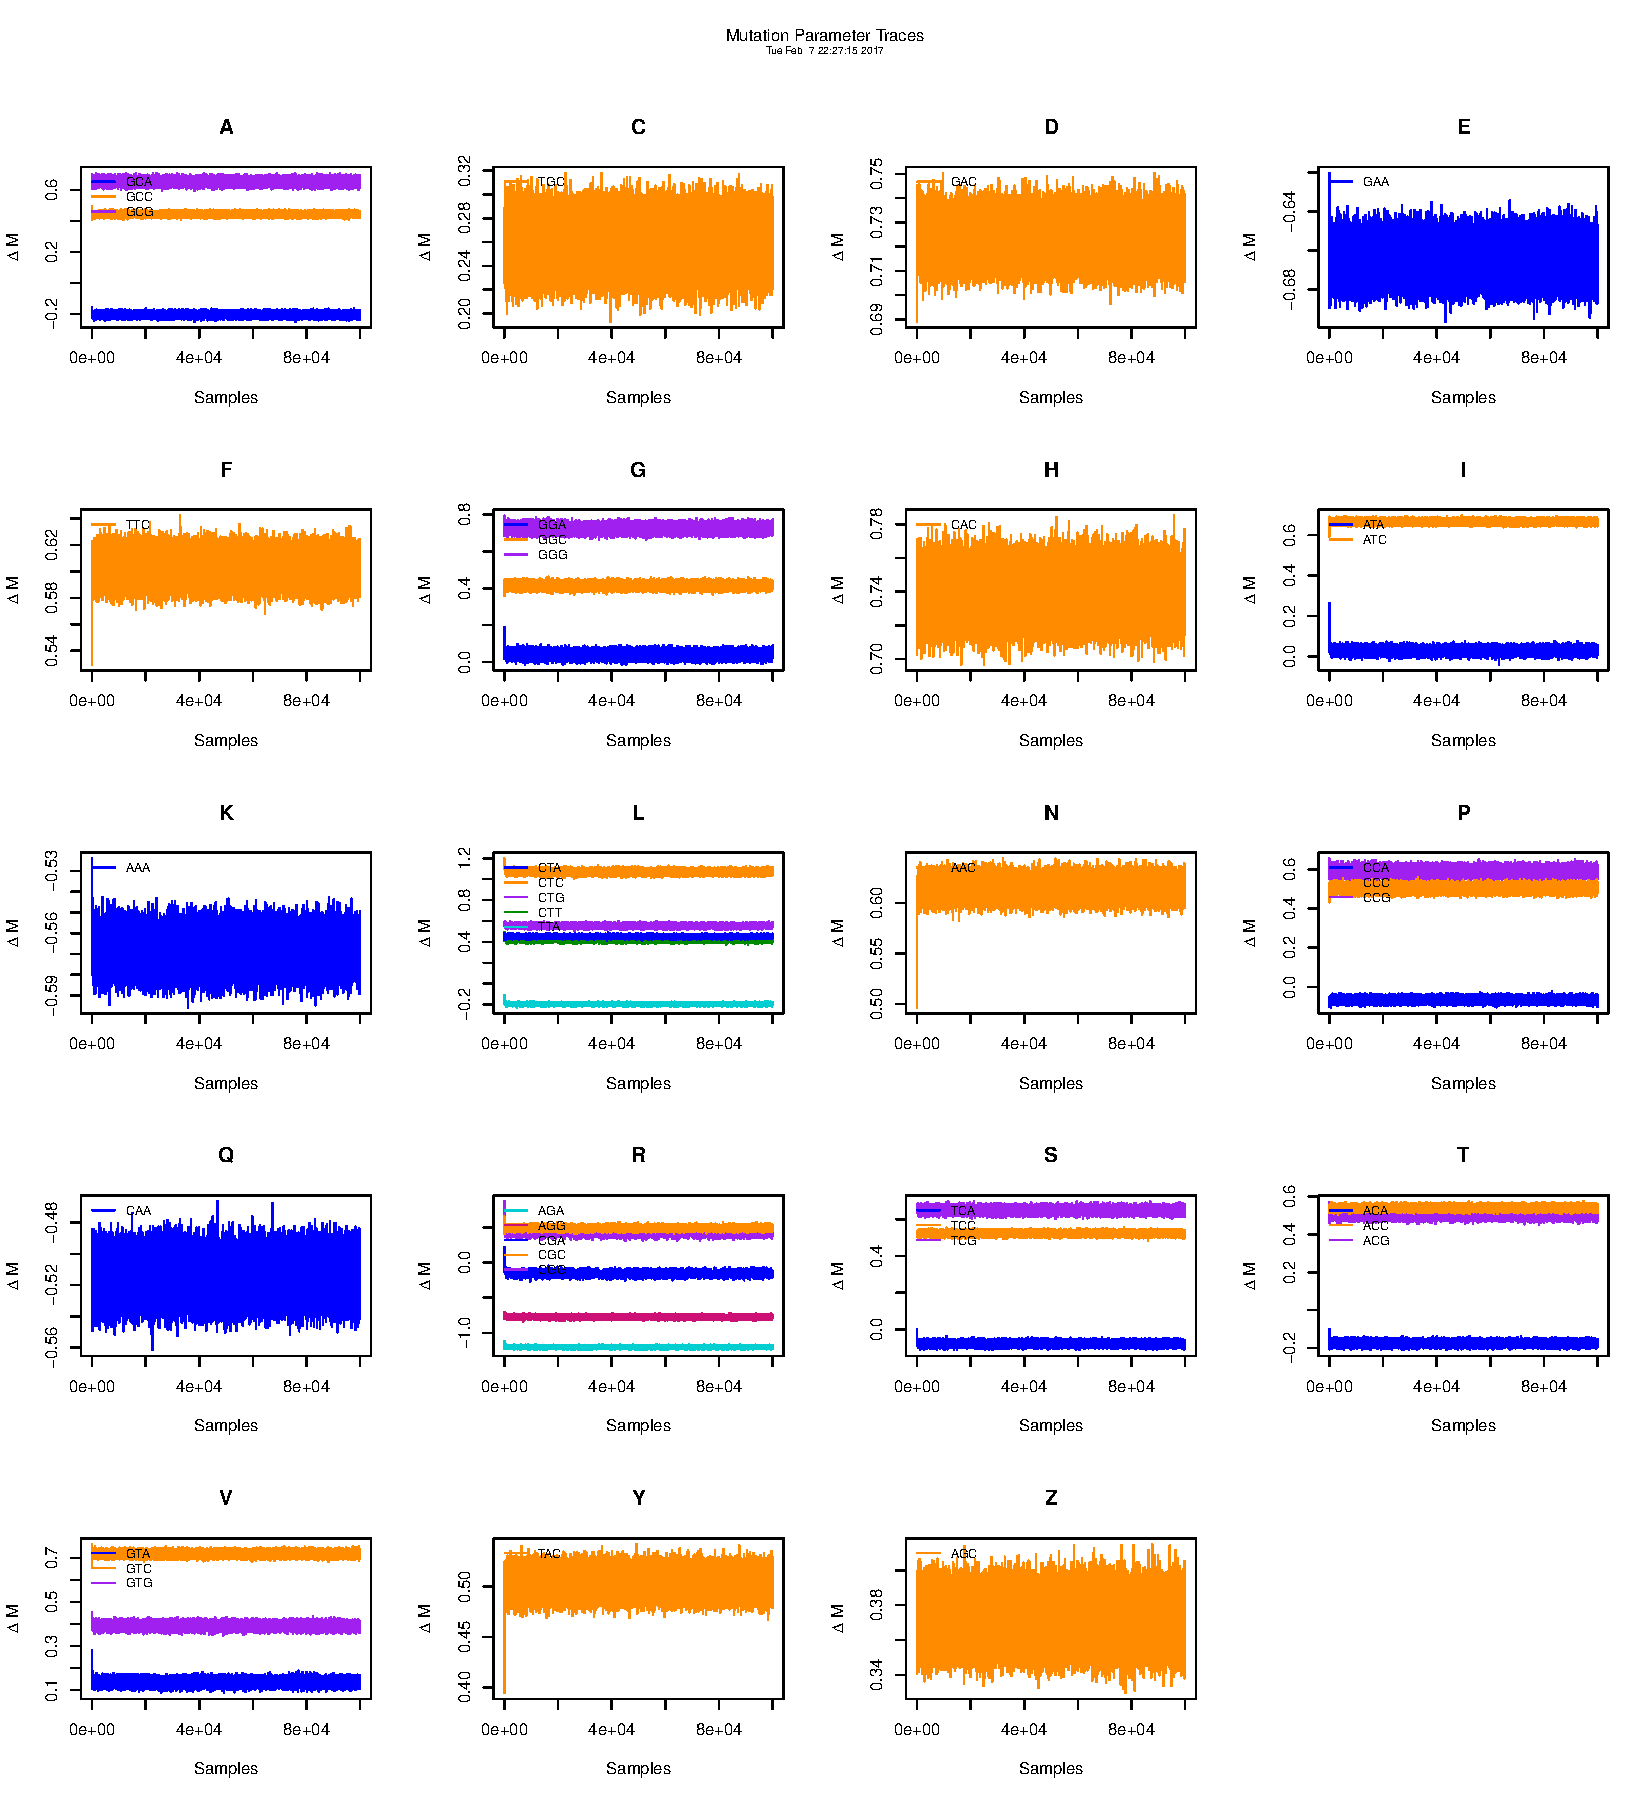
\includegraphics[page=1,scale=0.6]{Mixture_model_testing/Test_mixture/real_data/Graphs/yeast_deltaEta_deltaM_traces_CUB_plot_updated.pdf}
\caption{$\Delta\mathit{M}$ traces with mixture model for $\phi$}
\end{figure}

\begin{figure}[H]
\centering
\includegraphics[page=2,scale=0.6]{Mixture_model_testing/Test_mixture/real_data/Graphs/yeast_deltaEta_deltaM_traces_CUB_plot_updated.pdf}
\caption{$\Delta\eta$ traces with mixture model for $\phi$}
\end{figure}

\begin{figure}[H]
\centering
\includegraphics[page=3,scale=0.6]{Mixture_model_testing/Test_mixture/real_data/Graphs/yeast_deltaEta_deltaM_traces_CUB_plot_updated.pdf}
\caption{CUB plot with mixture model for $\phi$}
\end{figure}

\begin{figure}[H]
\centering
\includegraphics[page=1,scale=0.6]{Mixture_model_testing/Test_mixture/real_data/Graphs/yeast_logPost_mixProb_phi_traces_updated.pdf}
\caption{Log(Posterior Probability) trace with mixture model for $\phi$}
\end{figure}

\begin{figure}[H]
\centering
\includegraphics[page=9,scale=0.6]{Mixture_model_testing/Test_mixture/real_data/Graphs/yeast_logPost_mixProb_phi_traces_updated.pdf}
\caption{Expected value of $\phi$ trace with mixture model for $\phi$}
\end{figure}


\experiment{1-11-2017}
\textit{Meeting with Mike}
Likelihood ratio tests for treating them as same categories vs together. \textbf{Question: From a statisical philosophy point of view, can you take parameters estiamted in a Bayesian context and apply Frequentists/Classical hypothesis testing?} Fit model to mature peptides + pseudo-mature peptides. Compare confidence intervals. See if they overlap. Look up Deviance Information Criterion, might be useful here. Do the same thing for pseudo-signal peptides. 

Redo runs from before, but let diverge for about 100 iterations. Do traces converge to same spot. This gives confidence that our parameter estimation is correct.

Add function for calculating autocorrelation for different traces to package.

\textit{C. bescii} looks like it hasn't converged, so just run for longer. \textbf{It's interesting to me that $\Delta\eta$ and $\Delta\mathit{M}$ values for \textit{C. bescii} seem to be struggling to converge, where as \textit{E. coli} seems to have no problems. These are both prokaryotic organisms. Why would they be so different?} 

\subexperiment{Plan Going Forward}


\experiment{1-16-2017}
Re-ran ROC treating non-signal peptide genes and mature peptides as separate regions, but this time MCMC was allowed to diverge for 100 steps. Comparisons of $\Delta\eta$ values can be seen below. Clearly, the divergence had almost no impact on the parameter estimates, giving confidence that these results are likely correct. 

\begin{figure}[H]
\centering
\includegraphics[page=1,scale=0.6]{Ecoli_results/Nosp_w_mp_cat_divergence_100/Graphs/Comp_nosp_no_divergence_to_divergence_100.pdf}
\caption{Comparison of $\Delta\eta$ estimates in non-signal peptides genes when MCMC not allowed to diverge vs allowed to diverge for 100 steps}
\end{figure}

\begin{figure}[H]
\centering
\includegraphics[page=1,scale=0.6]{Ecoli_results/Nosp_w_mp_cat_divergence_100/Graphs/Comp_mp_no_divergence_to_divergence_100.pdf}
\caption{Comparison of $\Delta\eta$ estimates in mature peptide regions when MCMC not allowed to diverge vs allowed to diverge for 100 steps}
\end{figure}

\experiment{1-18-2016}
Ran pseudo-mature peptides with actual mature peptides as separate categories. 



\textit{Meeting with Mike}
1) Make divergence more robust, if it puts you in realm of underflow or overflow, either go back a step and stop (produce warining) or step back and keep proposing something until numerically valid range. \newline
2) Find reference for rejection sampling, look back at Wikipedia sources \newline
3) Work on wrapping head around model comparisons \newline
4) Compare posteriors when treating sp and mp as the same thing \newline
5) Compare yeast to benchmarks, should be in testing \newline
6) Don't worry about initial conditions being worried about single lognormal distribution \newline
7) Fit mixture model to real data, simulate based on true value, fit to simulated data, do not expect much divergence. Then try with old approach. Expect values to climb. \newline
8) How do confidence intervals for signal peptides and pseudo - signal peptides overlap? \newline


\experiment{1-25-2017}
Reference for rejection sampling: "Generalized Accept–Reject sampling schemes", Casella et al, Institute of Mathematical Statistics Lecture Notes, Monograph Series \newline

Performed Likelihood Ratio tests for Mature Peptide and Signal Peptide, which indicated significance at significance level 0.005 (critical value 66.7659). However, this is also true of Non-signal peptide genes treating mature peptides as same or separate category (290). Ran only non-signal peptide genes, split into two cateogories of equal size, and compared this to previous run treating non-signal peptide genes as one cateogry using Likelihood ratio test. This again indicates significance (180). \newline
 
Compared yeast. Need to simulate genome, run with model.

\subexperiment{Lab meeting}
Cedric is trying to get at idea where C Left originated. Basd estimates off of Rocus tree. 

Calculate effective sample size (ESS), Coda in R. Look into ESS. Want around 500 for every parameter. Start with CSP parameter. After that what are ESS for acf. 

Take over autocorrelation stuff. Say thinning is 10. Run for longer, how do confidence intervals change? Do they grow? 

\subexperiment{Math Eco Seminar - Preface and Chapter 1}
The "best" model is constrained by the types of models you are considering. 

 
 
For acf, for phis, calculate average and std pf autocorrelations and plot these. Cedric saw some autocorrelation of the autocorrelation. How well does posterior probability trace autocorrelation reflect autocorrelation with other parameters (genome and CSP parameters). Alternatively, look at effetive samples sizes for the different parameters. 

\experiment{2-1-2017}
Autocorrelation

Effective sample size for posterior trace using Ecoli full genome, 5000 samples, 50 thinning, was roughly 35. 

Average effective sample size of phi traces 

Make sure burn-in is thrown out, add 95\% confidence intervals.


For acf, modify acceptance-rejection target, lower rate, expect greater independence. Possibly add code to stop after achieving some level of ESS. Also could start independent chains, let diverge, do they converge to the same value. 

Brian says not to change acceptance-rejection target, probably won't change much.


Looked at DIC for Mature peptides and Signal Peptides, and Pseudo Signal Peptides and Real Signal Peptides.

DIC for MP = SP: 269364.2
DIC for MP != SP: 268584.8

DIC for PSP = RSP: 88066.73
DIC for PSP != RSP: 87887.16

In both cases, DIC is lower for alternative model. However, DIC tends to favor models that are overfitting.

Ando (2007) notes some problems with DIC. It is assumed that parameteric family of probability distributions that generate future observations encompasses the true model, which is not actually the case. Observed data are used to both construct posterior distribution and to computer the posterion mean of expected loglikelihood, which results in underestimating the bias. Same data used twice in calculating number of effective parameters.

Ando proposed BPIC

Do 100K run for phi mixture model. Look at simulated genome. Take last half of current parameter traces.


\experiment{2-2-2017}
Began phi mixture run using 100000 samples for yeast. Also started 40000 sample run for E. coli for purposes of looking at effective sample size (ideally want around 500 samples for everything). Tried to further understanding of PBIC, but still not quite sure how to implement. Finished reading Chapter 3A for seminar presentation. Got first draft of ASMS abstract to Bob. Want to have submitted before 5 tomorrow.

\experiment{2-3-2017}
Large portion of day was spent editing the ASMS abstract. Bob really wanted me to include results for C. bescii and C. thermocellum, but I'm still not convinced about the reliability of these results. We spun this so that validation of the results is on-going. Talked with Suresh about getting some gene expression data for C. bescii, but he says the results have still not been processed and likely won't be useable at the moment. I found some C therm RNASeq results produced by the Steve Brown lab at ORNL, but it looks like these use different identifiers. Will need to find mapping.

I remembered today that I need to re-run some of the E. coli fittings with divergence. Cedric said he usually allows divergence for 10 iterations. 


\experiment{2-5-2017}
Spent part of today cleaning up and testing some code (stuff for ACF I wrote that will be added to the repository. Looks like I need to fix the $S_\phi$, $\epsilon$, $M_\phi$ hyperparameter plots for the  $\phi$ mixtures. Also need to update reading and writing restart files and Robjects to account for changes in code (such as save likelihood, etc.)

\experiment{2-6-2017} 
Got around to looking at results of E.coli fittings with divergence. Patterns for $\Delta Eta$ correlated well, but the slope deviated significanlty from 1 (roughly 0.5). This was certainly concerning and I began digging into the code in order to find out what was going on. I had previously allowed divergence for 100 iterations when fitting the non-signal peptide genes and mature peptides, but this did not result in the strange behavior I was currently seeing. I checked some of the previous updates to ROC to make sure none of the changes would cause these strange results Eventually, I realized the problem was in the varyInitialConditions() function in MCMCAlgorithm module. This function varies everything, even parameters not being estimated. This would be problematic in the cases where I do not estimate phi, such as runs where I fit to the mature peptides and signal peptides. By allowing the $\phi$s to diverge, I'm effecitively shifting the search space for the algorithm and it has no chance to get back to that space because $\phi$s will not be changed after the initial divergence. 

\experiment{2-7-2017}
Spent most of the day preparing for Math Eco seminar. Also assisted with Darwin Day. Tried simulating Yeast genome, but I got an error when I tried to load the saved parameter object. I will need to fix this before I can proceed further. Need to fix restart files and R objects issues before I proceed further. This will save me time in the future.  
 
\experiment{2-8-2017}
Realized I made a mistake in changing varying initial conditions. Somehow, I accidentally deleted the for loop in this function, so I need to redo the runs I did previously; however, I expect results should still be consistent with results that don't allow divergence. 

\subexperiment{Gilchrist Lab Meeting} 
Run DIC calculations on PseudoMp-Mp runs. 


\experiment{2-9-2017}
Made edits to Bioinformatics paper based on Mike's comments. Pushed to directory

\experiment{2-10-2017}
New functions for plotting posterior and likelihood seem to be working. Need to test on case where don't estimate expression. Will not modify code to update these terms when estimating hyperparameters. Seems unlikely there would ever be a case when someone wants just these parameters and to keep everything else constant. 

\experiment{2-12-2017}
Was testing something with my old implementation of the $\phi$ mixture model to make sure the hyperparameters were being updated. Noticed both epsilon terms were staying at 0. This might partially explain why results from that second run looked decent.



\experiment{2-13-2017}
\subexperiment{$\phi$ Mixture Model Math Notes}

Want to be able to represent $\phi$ estimates as mixture of two distributions to more accurately reflect empirical data. Typically, gene expression data appears bimodal, with the a distribution 


\experiment{2-20-2017}
\subexperiment{Meeting with Bob}

SIPROS - home built version of MiriMatch, allows for isotopic labeling 

We know the Adams and Kelly groups, so we can contact them if necessary. 


\experiment{2-22-2017}

I've been thinking about the divergence problem for MCMC. Goal was to make it if overflow or underflow occurred while diverging, then go back to the previous state and re-sample the parameters. This would be easy enough if dealing with unsigned or signed integers. If unsigned, the output is defined in C++. Signed integer arithmetic is not well-defined, but typically overflow will result in two positive numbers summing to produce a smaller number and underflow will result in two negative numbers summing for a positive. This would be very easy to detect. The problem is we are dealing with floats/doubles. The way these are defined by IEEE allows for gradual overflow or underflow. What this means is overflow/underflow will not occur the moment you 


\experiment{2-27-2017}
Make plots of phis for each segment - how do they vary
Plot uncertainty for all of the fits through the origin
Maybe can just initialize value and not estimate hyperparameters. Also reduce $s_\epsilon$ by an order of magnitude. 

Plot estimates of slope and intercept, how do they vary? We want to be able to tell if slope differentiates from 1 and if intercept differentiates from 0. How do confidence intervals vary from 1 and 0 (plot these lines, do they overlap). 

For Ctherm, check ribosomal genes are. Ideally, indicate where they are in CUB-expression plot histogram
Create histrograms of deltaEta and deltaM, grouped by third nucleotide for 2 codon amino acids only.  

Plot histogram of differences for delta etas. 

Start looking at journals for signal peptide paper for E.coli.  

\experiment{3-7-2017}
Potential journals for signal peptide paper
\begin{itemize}
	\item Biochemical and Biophysical Research Communications
	\item Nucleic Acids Research
	\item Trends in Microbiology
	\item BMC Genomics
\end{itemize}

\experiment{3-8-2017}

\textbf{Documentation to edit for ribModel package}
\begin{itemize}
	\item convergence\_test.Rd
\end{itemize}


\experiment{3-14-2017}

\subexperiment{Histogram of Phis by segment for \textit{E. coli}}
\includepdf[pages=-]{Ecoli_results/Segments_expression/Histograms_phis_by_segment.pdf}


\experiment{3-16-2017}

\subexperiment{Divergence iterations numerical errors}
Initial testing seems promising. Initialized all CSP parameters to 1000, which resulted in numerical errors in the $\phi$ estimates, which was reported by the code. Similarly, if CSP are started near the upper bound of floating point representation ($10^308$), numerical errors are achieved and reported. The code is able to report these warnings during the divergence steps. One interesting behavior about R is it does not allow gradual overflow, meaning anything greater than or equal to $10^308$ will be set as infinity, but gradual underflow is allowed, meaning you can go lower than $10^-308$. I'm concerned about how this will impact the software because C++ does allow for gradual overflow. 

\subexperiment{Signal Peptide Project}
Took a closer look at some of the $\Delta\eta$ confidence intervals for the signal peptides and pseudo-signal peptides. It looks like quite a few of them overlap with 0, which means we can't be certain which is the optimal codon. I don't think this changes the overall story, but I would rather eliminate any sources of possible doubt in our analysis. 

\experiment{3-22-2017}
\subexperiment{Gilchrist Lab Meeting}

\textbf{Things to do:}
\begin{itemize}
	\item Register for SMBE (how to get reimbursement?)	
	\item Start at true values as point of comparison for phi mixture
	\item Start multiple runs for phi mixture, make sure they all converge  
	\item Dealing with gradual overflow/underflow between C/C++
	\item Histogram of simulated phi values, do we see a distinguishable hump?
	\item pull out ribosomal genes for histogram and plot those for both empirical and estiamted phis in Ctherm.
	\item For likelihoods, maximize $x^*$ for some a and b such that $y^* = bx^* + a$, is it better than some other set of a and b.
\end{itemize} 

\experiment{3-27-2017}
\subexperiment{Hettich Lab Meeting}
Discussed HUPO meeting Bob was at last week. 

DiLu - new software for identification of high resolution of metabolomics data \newline

\textbf{Single-Cell Mass Spectrometry for Discovery Proteomics: Quantifying Translational Cell Heterogeneity in the 16-Cell Frog (\textit{Xenopus}) Embryo}\newline

Capillary electrophoresis (CE) has traditionally had poor dynamic range (3 log orders in this paper, our work is usually between 6 and 7). 

For CE-$\mu$ ESI had surprisingly high charges (4-6)

emPAI is a relative abundance metric.  

\experiment{3-29-2017}
Cedric implemented HMM, looks like it's working, but trying to speed it up. Trying to solve matrix exponentiation problem in a more computationally efficient manner. 


\experiment{3-30-2017}

Self-assessment following colloquium presentation
\begin{itemize}
\item During questions, don't provide sassy answers. Keep it professional.
\item Make it more clear what the purpose of the research is, why people should care
\item Thanked Mike and Bob. During formal presentation, should thank Dr. Gilchrist and Dr. Hettich
\item Mentioned statistical significance by using likelihood ratio tests, but my audience was likely not familiar with this
\item Don't pace so much and keep your eyes on the audience
\end{itemize}

\experiment{4-3-2017}
Fixed problem with plotParameter.R module. Seemed to be always plotting the confidence intervals. Now fixed and needs to be pushed. Also eliminated "estim.Expression" parameter in plotModel.R

Looked at mature peptides and signal peptide regions in \textit{E. coli} O157:H7. Results actually look generally cleaner than \textit{E. coli} K12. 


\includepdf[pages=2]{Ecoli_O157_results/Mp_w_sp_cat/Graphs/ecoli_mp_w_sp_cat_traces.pdf}

Checked out a signal peptide database found at http://www.signalpeptide.de. For \textit{E. coli} K12, there are 155 confirmed signal peptides, 9 indicated determined to be signal peptides by similarity, 8 indicated to be probable, and 327 potential signal peptides. 

\experiment{4-5-2017}
NIMBioS workshop on August 7th - August 11th.
Check out Halpern and Bruno, 1998.
Register for SMBE and make hotel reservations.
\subexperiment{Gilchrist Lab Meeting}
\textbf{To do:}
\begin{itemize}
\item Generate segment histograms for segments on the same graph. Potentially rescale $\Delta\eta$s  
\item Re-do runs for segments, fix sphi to value estimated. 
\item So look at other strains of \textit{E. coli} 
\end{itemize}

\subexperiment{Mike's Feedback on Colloquium Presentation}
\begin{itemize}
\item Overall very good
\item Figures axes labels were too small. 
\item We do have an idea. Don't say we don't. 
\item What is going on with plateuing of $\Delta\eta$ values? If we have saturated information, then we struggle with identifiability
\end{itemize}

\experiment{4-10-2017}

Things Mallory needs:
\begin{itemize}
\item Needs a list of MS1 peak lists with intensities
\item Needs a separate output with scan number and file name to index with MS1 peaks
\item For matrix, put file names at top instead of file index
\item During processing, throw out any peaks also found in blank or control. Can do this post-processing wise. 
\end{itemize}

\textit{C. bescii} has an Arginine codon that never seems to converge for the $\Delta\eta$ parameter. Seems this codon never occurs in this region of the genome. How might this impact interpretations of these results. 

\experiment{4-11-2017}
Potential dates and times for first committee meeting.

\begin{itemize}
\item May 1, 9 - 10 am
\item May 1, 10 - 11 am
\item May 1, 11 am - 12 pm
\item May 1, 12 - 1 pm
\item May 1, 1 - 2 pm
\item May 1, 2 - 3 pm
\item May 8, 11 am - 12 pm
\item May 8, 12 - 1 pm
\end{itemize}

\experiment{4-12-2017}
After examining previous runs, arginine codons AGA and AGG consistently seem to be the ones that diverge the most from the $y = x$ line in runs looking at the front of genes vs the end of genes. tRNA copy numbers for these genes are as follows according to: \newline http://lowelab.ucsc.edu/GtRNAdb/Esch\_coli\_K12

\begin{itemize}
\item CGT - 4 
\item CGC - 0
\item CGG - 1
\item CGA - 0
\item AGG - 1
\item AGA - 1
\end{itemize}

This is interesting because both CGC and CGA are preferred over their counterparts AGA and AGG, which both have a tRNA copy number of 1. 

Noted that \textit{E. coli} O157:H7 (Sakai) strain had more linearly correlated relationship and was closer to $y = x$ than \textit{E. coli} K12 MG1655 strain. Interestingly, I found paper that found that \textit{E. coli} O157:H7 (Sakai strain) had a 2-fold enrichment of the AGA tRNA gene, which was one of the problematic ones in \textit{E. coli} K12 MG1655. With wobble, would this also make AGG more viable? Also, some organisms use AGA and AGG as a non-canonical stop codon. Is it possible that that \textit{E. coli} either does this (haven't found anything yet) or evolved from a bacteria that once used these as non-canonical stop codons? 

To do list:
\begin{itemize}
\item Download Uniprot database. Figure out signal peptides
\item 5-10 gram-positive bacteria and 5-10 gram-negative bacteria
\end{itemize}


Notes on Newton:
Taking nodes from Newton less than 4 years old, going to make part of larger set of clusters. Improves access to computational resources. Will be taken down in June.


\experiment{4-13-2017}

Gram-positive bacteria
\begin{itemize}
\item \textit{C. thermocellum}
\item \textit{S. aureus}
\item \textit{S. sobrinus}
\item \textit{B. clausii}
\item \textit{M. tuberculosis}
\item \textit{S. pneumoniae}
\item \textit{S. coelicolor}
\end{itemize}
 
Gram-negative bacteria
\begin{itemize}
\item \textit{E. coli}
\item \textit{C. bescii}
\item \textit{M. luteus}
\item \textit{V. cholera}
\item \textit{P. aeruginosa}
\end{itemize}

\experiment{4-17-2017}

Mallory and I discussed the potential of clustering metabolmics data based on MS1 and MS2 Peak intensity in fashion similar to MET-COFEA and MS-CLUSTER algorithms. If we are able to do so and perform analysis that shows this is a valid approach for metabolites, might be worth a paper. 




\experiment{4-19-2017}

\subexperiment{Gilchrist Lab Meeting}
To Do:
\begin{itemize}
\item Time Tree, Tree of Life 
\item Ben Fitzpatrick might be a good person to talk to
\item Mike is meeting with Philip Myer, over in Ag. Campus interested in heratibility of microbes/metabolites in cattle on April 28th quantitative genetics and metabolomics of microbiome
\item For later, find expression datasets for microbes we are interested in.

\end{itemize}


\experiment{4-21-2017}
Look into opportunistic bacterial pathogens. These pathogens depend on certain environmental factors that allow these bacteria to become pathogens. Often times can be controlled by a more dominant bacteria in the environment that prevent dangerous bacteria from grabbing a foothold.

Many fungi do not operate at 98.6 F, hence why we do not always have fungal infections.  

\experiment{4-26-2017}

Median times of divergence according to TimeTree.org
\begin{itemize}
\item E. coli to B. clausii - 3169 MYA
\item E. coli to Cauldicellulosiruptor bescii - 3169 MYA
\item E. coli to C. thermocellum - 3169 MYA
\item E. coli. to M. luteus - 3169 MYA
\item E. coli to M. tuberculosis - 3169 MYA
\item E. coli to Pseudomonas aeruginosa - 1438.8 MYA
\item E. coli to Staphylococcus aureus - 3169 MYA
\item E. coli to Streptomyces coelicolor - 3169 MYA
\item E. coli to Streptococcus pneumoniae - 3169 MYA
\item E. coli to Streptococcus sobrinus - 3169 MYA
\item E. coli to Vibrio cholerae - 842.2 MYA
\item B. clausii to C. bescii - 2650 MYA
\item B. clausii to C. thermocellum - 2650 MYA
\item B. clausii to M. luteus - 3077 MYA
\item B. clausii to M. turberculosis - 3077 MYA
\item B. clausii to P. aeuruginosa - 3169 MYA
\item B. clausii to S. aureus - 1558 MYA
\item B. clausii to S. coelicolor - 3077 MYA
\item B. clausii to S. pneumoniae - 1810 MYA
\item B. clausii to S. sobrinus - 1810 MYA
\item B. clausii to V. cholerae - 3169 MYA
\item C. bescii to C. thermocellum - 1997 MYA
\item C. bescii to M. luteus - 3077 MYA
\item C. bescii to M. tuberculosis - 3077 MYA
\item C. bescii to P. aeruginosa - 3169 MYA
\item C. bescii to S. aureus - 2650 MYA
\item C. bescii to S. coelicolor - 3077 MYA
\item C. bescii to S. pneumoniae - 2650 MYA
\item C. bescii to S. sobrinus - 2650 MYA
\item C. bescii to V. cholerae - 3169 MYA
\item C. thermocellum to M. luteus - 3077 MYA
\item C. therm to M. tuberculosis - 3077 MYA
\item C. therm to P. aeruginosa - 3169 MYA
\item C. therm to S. aureus - 2650 MYA
\item C. therm to S. coelicolor - 3077 MYA
\item C. therm to S. pneumoniae - 2650 MYA
\item C. therm to S. sobrinus - 2650 MYA
\item C. therm to V. cholerae - 3190 MYA
\item M. luteus to M. tuberculosis - 1645 MYA
\item M. luteus to P. aeruginosa - 3169 MYA
\item M. lutues to S. aureus - 3077 MYA
\item M. luteus to S. coelicolor - 1645 MYA
\item M. luteus to S. pneumoniae - 3077 MYA
\item M. luteus to S. sobrinus - 3077 MYA
\item M. luteus to V. cholerae - 3169 MYA
\item M. tuberculosis to P. aeruginosa - 3169 MYA
\item M. tuberculosis to S. aureus - 3077 MYA
\item M. tuberculosis to S. coelicolor - 1278.1 MYA
\item M. tuberculosis to S. pneumoniae - 3077 MYA
\item M. tuberculosis to S. sobrinus - 3077 MYA
\item M. tuberculosis to V. cholerae - 3169 MYA
\item P. aeruginosa to S. aureus - 3169 MYA
\item P. aeruginosa to S. coelicolor - 3169 MYA
\item P. aeruginosa to S. pneumoniae - 3169 MYA
\item P. aeruginosa to S. sobrinus - 3169 MYA
\item P. aeruginosa to V. cholerae - 1438.8 MYA
\item S. aureus to S. coelicolor - 3077 MYA
\item S. aureus to S. pneumoniae - 1810 MYA
\item S. aureus to S. sobrinus - 1810 MYA
\item S. aureus to V. cholerae - 3169 MYA
\item S. coelicolor to S. pneumoniae - 3077 MYA
\item S. coelicolor to S. sobrinus - 3077 MYA
\item S. coelicolor to V. cholerae - 3169 MYA
\item S. pneumoniae to S. sobrinus - 0.797 MYA
\item S. pneumoniae to V. cholerae - 3169 MYA
\item S. sobrinus to V. cholerae - 3169 MYA
\end{itemize}

As a reference point, humans and chimps diverged about 6.4 MYA and mice (Mus musculus) and humans diverged about 88 MYA. 

For some reason, ROC breaks in the initialization of the covariance matrix for M. luteus. 


\subexperiment{Gilchrist lab meeting}
Add segment analysis for other microbes. Note that pathogenic bacteria who are mainly host-driven (can only really thrive in context of host) have smaller effective population size, which will dampen the effects of selection. Might want to expand analysis to include more non-pathogenic microbes. Use errors-in-variables regression slopes, not regular regression slopes.


\experiment{4-28-2017}

\subexperiment{Meeting with Dr. Phillip Myer Animal Sciences}

\textbf{Background} Interplay of factors such as diet management, host genetics, and GIT microbiome are key factors in the nutritional status of beef cattle. Current knowledge of the effects of GIT microbial population dynamics on host productivity is insufficient. Myer's research is focused on mechanisms explaining differences in feed efficiency in beef cattle, nutrition of grazing beef cattle and interactions with the ruminal and lower GIT microbial communities, and the establishment of the rumen microbiome and its effects on growing beef cattle. 

Ruminants are mammals that can acquire nutrietns from plant-based food by fermenting it in a specialized stomach prior to digestion, mainly through microbial actions. The rumen is first chamber in the GIT of ruminants and serves as the primary site of microbial fermentation. 

Wants to optimize feed efficiency. Feed less, gain more for cattle. Interested in how to optimize at the microbiome level in Tennessee. Cow gives birth, weened, ends up being sent to larger pasture area such as Nebraska. Here we are mainly birthing and growing cattle. To what degree do microbes affect the host, to what degree does the host affect the microbiome? Wants to think about just inheritability. Was considering a twin-study, but USDA was not a fan, so just drop it. What are the best microbes to optimize them while they are here in Tennessee. Basically, want to look at the heritability of the microbiome. Intake vs weight. Efficiency is broader impact, but heritability is Myer's main interest for this study. There are heritability measures, but the problem is he wants to treat the microbiome as a trait to inherit. Have access to tools for metabolomics, metagenomics, and (maybe) transcriptomics. Dr. Brynn Voy will be on this study as well. Will be untargeted metabolomics data. Will run rumen and serum metabolomics. Fatty acids might be of particular interest. There are plenty of physiological factors that we might be able to look at. Look into Turnbaugh who has done quite a bit of work on human microbiome heritability. In regards to cattle, Paul Weimer up at University of Wisconsin. For beef cattle, still largely in characterization phase (looking for genetic markers). Grant is due June 15th. Will need to be done way before that. 

For metagenomics, will use traditional sequencing or amplicon sequencing (16s rRNA genes) for more targeted analysis. In Rumen, 0.02 or fewer sequences are unidentifiable, but 0.8 of bacteria are unculturable. Mike thinks we might be able to use CUB as a signature for differentiating between sequence sources. GreenGenes, Silva, NCBI's database, RDB (ribosomal database). 


\experiment{5-3-2017}

V. cholerae O1 El-Tor is genetically different from the classic strain, but can still live in water (does not necessarily have to be in human host to thrive).

S. aureus NCTC 8325 is known for causing skin conditions.

S. pneumoniae is apart of normal upper respiratory tract and can become pathogenic under the right conditions.

M. tuberculosis is only known to thrive in humans and some evidence suggests different strains co-evolved with local human population.

B. clausii is a soil bacteria.

S. sobrinus is pathogenic to humans and can be found in cavities/plaque in the human mouth.

S. coelicolor is a soil dwelling bacteria.

C. bescii and C. thermocellum are both cellulolytic thermophiles. 

P. aeruginosa can be found in various environments (soil, water, skin, and man-made environments). Is pathogenic. Not as virulent as other pathogenic bacteira. 

Microcystis aeruginosa is freshwater cyanobacteria and is Gram-negative. 

G/C content
\begin{itemize}
\item B. clausii - 44.8 - aerobic
\item C. bescii - 35.2189 - anaerobic
\item C. thermocellum - 39.1 - anaerobic
\item E. coli - 50.8- facultative anaerobic 
\item M. tuberculosis - 65.60 - aerobic 
\item P. aeruginosa - 66.60 - facultative anaerobic
\item S. coelicolor - 71.982 - aerobic 
\item S. aureus - 32.9 - facultative anaerobic
\item S. pneumoniae - 39.7 - facultative anaerobic
\item S. sobrinus - 43.4 -  anaerobic
\item V. cholerae - 47.4873 - facultative anaerobic
\end{itemize}

\experiment{5-10-2017}
Email correspondence with Dr. Tessa Burch-Smith. Is interested in performing a meta-analysis of publicly-available microarray and RNA-Seq data. Specifically, they want to look at expression of different classes of cell-wall and reactive oxygen species-related genes on response to different treatments and use that as a guide to test our hypotheses. Meeting is tenatively scheduled for June 12th at 1pm.


\subexperiment{Meeting with Annabel}
At lower temperatures, find bigger protein clusters. Varying protein-lipid interaction term. At lower temperatures, as increase $J_{PL}$ smaller. Did not try to modify $J_{LL}$ interactions, Steve thought it best to keep these constants. Might also want to modify $J_{PP}$ interactions. Annabel would like to see this project to the end, despite her being way. Helped Rob with antigen-bonding projects. Project is now with multiple bonds.  


\begin{itemize}
\item investigate whether protein-lipid interaction energy affects phase separation of lipids at 300K.
\item Varying protein-protein interaction energy and observe how this affects the system.
\end{itemize}



Annabel will be working with Dan Jacobson for two terms at ORNL (next spring and next summer). Also will be working out at Berkeley before that. 


\experiment{5-17-2017}
\subexperiment{Gilchrist Lab Meeting}
Implemented likelihood profiling approach for getting confidnece intervals for errors-in-variables approach. Performed parametric bootstrap for both Pearson and Spearman correlation coefficient, but confidence intervals were both lower than the calculated metric, which seems wrong. Needto double check code and estimates used.

MetSign author is not replying to emails. Need to use different software. Potentially MS-Cluster, recognizing this tool was developed for proteomics, not metabolomics. Will likely need another software for data pre-processing to filter out noise. 

Work from the Wilke group might not be appropriate because from different isolate of \textit{E. coli}. Microarray data from the systems biology group seems appropriate. Has many experiments with K12 MG1655 strain under different conditions. Look into E. coli strain presented by Wilke group. How do results differ, if at all, from K12 MG1655 strain. 

\experiment{5-24-2017}

Wrapping up stuff with Mallory prior to ASMS

First-order and second-order approximation stuff is on RibModelDev. Maybe work with undergrad on FONSE work.

Take a look at site-dependent PNAS paper. If I find it interesting, send to Mike  

Look into Qin paper

\includepdf[pages=-]{Ecoli_results/codon_changes.pdf}

\experiment{6-12-2017}
\subexperiment{\textit{E. coli} gene expression in response to glucose starvation}
See \cite{houser2015} for details.

Focuses on \textit{E. coli} B REL606 in the stationary phase in response to glucose starvation. 

Monitor both RNA and protein responses over course of two weeks. \textbf{Limit mRNA and protein production}, degrade proteins involved in energy-intensive processes, and maintain or increase the amount of proteins involved in energy production. 

Also examine lipid and flux metabolic analysis. 

mRNA counts normalized via DESeq relative to total pool of mRNA, tRNA, and ncRNA. Protein counts were likewise normalized via total protein counts. Used K-means clustering on mRNA and proteins shown to be changing significantly. Approx. 1900 transcripts/proteins after applying this filter. mRNAs were generally down-regulated, but proteins were more varied. After starved state was entered, transcription profiles remained relatively constant.  
 
Absolute abundance values for proteins and RNA at 3 hour time point had Spearman correlation coefficient of 0.71 

Hierachical clustering showed trends in down and up regulated RNA and proteins based on GO terms. RNA down-regulated included translation, cellular cell wall metabolic process, nitrogen compound biosynthetic process, aerobic respiration. and nitrogen compound biosynthetic process. RNA up-regulated was carbohydrate catabolic process. Down-regulated are likely for energy conservation. Protein down-regulated included translation, cellular cell wall macro,olecule metabolic process, locomotory behavior, RNA modification. DNA-dependent DNA replication, and cell cycle. Protein up-regualted included lipid modification, carbohydrate catabolic process, response to osmotic stress, glyceral metabolic process, iron ion transport.

\subexperiment{The \textit{E. coli} molecular phenotype under different growth conditions}
See \cite{caglar2017} for more details.

Examines \textit{E. coli} B REL606 under 34 conditions. Consider both exponential and stationary phase cells. Alter concentrations of sodium and magnesium in growth media. Also examine different carbon sources: glucose, gluconate, lactate, and glycerol.

Growth phase had the greatest impact on systematic difference in mRNA abundance based on hierachical clustering. Results for protein abundance suggests sodium levels and carbon source have greater impact on shaping protein abundances. 


\experiment{6-14-2017}

Kullback-Liebler distance is the distance between the true model and your model. Could they potentially formulate SELAC and other models so they are nested, allowing employment of a likelihood ratio test. 

AICc under different conditions:
\begin{itemize}
\item number of sites
\item number of sites times number of taxa
\item number of taxa
\end{itemize}
Calculate AICc under all conditions, take one that fits best. 

Common rule for AIC is ratio of number of parameters to number of datapoints of about 40. 

Functionality in SELAC is currently a linear function. Reduce functionality by 3, then increase expression by 3, which is biologically unrealistic. Can we come up with another approach that might be based on the structure of the protein or physio-chemical properties of the individual amino acids. 

PhyloBayes.org has software that implements Halpern and Bruno 1998 model. Check out if you find the time. 

Hackathon for playing around with the Tree of Life August 8th through 11th. 

Look at credibility intervals for ribosome protein expressions in \textit{C. bescii} and \textit{C. thermocellum}.

\experiment{Signal Peptide Paper Outline}
Working title: \textbf{Assessing Codon Usage Bias as a potential marker of Signal Peptides in \textit{Escherichia coli}}

Authors: Alex Cope, Robert Hettich, Michael Gilchrist
\begin{outline}[enumerate]
\1 Introduction
	\2 Why is protein secretion importance
		\3 Many proteins important to biological processes are secreted
			\4 Anti-bacterial resistance proteins ($\beta$-lactamase)
			\4 Metabolism proteins (Maltose Binding Proteins, proteins in cellulolytic microbes - find specific examples)
			\4 Need to understand mechanisms of protein secretion
		\3 Pathways of protein secretion in Gram-negative bacteria
			\4 General Secretory Pathway - evolutionarily conserved across domains of life, common feature is signal peptide
			\4 Signal peptides have relatively consistent chemical properties, but some variation is possible (ex. effects of neutralizing N-terminus on secretion)
			\4 Summarize work suggesting signal peptides in \textit{E. coli} have bias for translation inefficient codons
			
	\2 Relevance of Signal Peptide prediction and other localization prediction software
		\3 MS can theoretically be used to measure the secretome
		\3 Problems with experimental approach: 
			\4 Low abundance proteins can be confused with noise
			\4 Cell lysis...how do you distinguish between actual extracellular proteins and cytoplasmic proteins in the sample from cell lysis
		\3 Use tools like SignalP and Psort to help distinguish between extracellular and cytoplasmic proteins in experimental results
			\4 Tools are also subject to error. How can we improve them? 
		
\1 Main Question
	\2 Does selection differ on the CUB of signal peptides in \textit{E. coli} compared to the rest of the genome? Is there selection for translation inefficient codons?
	\2 If so, then CUB could be a viable marker of signal peptides, allowing us to improve signal peptide prediction
\1 Methods
	\2 Tools: SignalP and ROC-SEMPPR
	\2 Describe how coding sequences are categorized (non-signal peptide gene, signal peptide, mature peptide)
	\2 Describe generation of pseudo-signal peptide genes
	\2 Describe how each coding sequence is segmented to analyze CUB and how it varies along a gene
	\2 Estimate $\Delta\eta$ via ROC-SEMPPR for various regions
\1 Results
	\2 Expected results given signal peptides are under seleciton for translation inefficient codons: Negative correlation bewteen $\Delta\eta$ parameters for signal peptides and mature peptides
	\2 Actual Results: Positive correlation between parameters
	\2 Comparison of signal peptides to first 25 codons of pseudo-signal peptide genes
	\2 See decline in slopes comparing $\Delta\eta$ estimates from 25 codons segment further down the genes to first 25 codon segment
		\3 Can also present traces of $\Delta\eta$ values for each codon for each segment
\1 Discussion
	\2 Positive correlation means direction of selection in signal peptides is consistent with the rest of the genome
	\2 CUB in signal peptides is most consistent with 5' ends of non-signal peptide genes, but still not the 1:1 ratio we were expecting...why?
	\2 See general decrease in slope over the length of coding sequences, consistent with selection against nonsense errors
	\2 Drop-off at end of slope trace is result of arginine codons AGA and AGG no longer being present
		\3 These two codons vary from the $y = x$ line, do not know why yet
		\3 AGG and AGA are non-canonical codons in mitochondria and some organisms...coincidence or suggest something biological about \textit{E. coli}?
	\2 Address contradictions with experimental work
		\3 Optimization of CUB can result in drops in expression (find references), which would explain experimental results
		\3 Experimental work required researchers to use different sets of translation ineffient codons to get consistent results. 
			\4 Only one of these sets was consistent with the bioinformatic analysis that jump started their research.
\1 Conclusion
	\2 Contrary to previous work, selection for CUB in signal peptides is consistent with rest of genome
	\2 CUB is likely not a good marker for signal peptides
	\2 Selection against nonsense errors likely one contributor to variation in CUB along genes in \textit{E. coli}, but others likely exist
            
\end{outline}

\experiment{6-21-2017}
\subexperiment{Comparing ROC-SEMPPR $\phi$ to RNA-Seq and Proteomics data from \cite{caglar2017}}

In general, raw mRNA counts \textbf{do not} correlate well with $\phi$ estimates of ROC-SEMPPR.
\begin{figure}[H]
\centering
\includegraphics[page=1,scale=0.6]{Ecoli_REL606/GSE94117_raw_mrna.pdf}
\caption{Comparison of raw RNA-Seq counts to ROC-SEMPPR $\phi$}
\end{figure}


By normalizing the RNA-Seq counts, correlations generally improve. I examined three normalization techniques:
\begin{itemize}
\item Reads Per Kilobases per Million Reads (RPKM) 
\item Transcripts Per Million (TPM)
\item size factors calculated by DeSeq2 (R package)
\end{itemize}

Let $r_g$ be the number of reads for gene $g \epsilon G$, $fl_g$ be the feature length - the number of nucleotides in a mappable region of a gene - and rl be the read length - the average number of nucleotides mapped per read. From my understanding $fl_g$ will be shorter than the length of the gene if dealing with things such as introns. Given that I am looking at a bacteria where introns are relatively rare, I just substituted in the length of the gene for $fl_g$.  
\begin{align}
RPKM_g &= \frac{r_g \times 10^9}{fl_g \times R} \\
R & = \sum_{g \epsilon G} r_g \text{(total number of reads from sequence run)}\\
TPM_g &= \frac{r_g \times rl \times 10^6}{fl_g \times T} \\
T &= \sum_{g \epsilon G} \frac{r_g \times rl}{fl_g} \text{(proxy for number of transcript samples)}
\end{align}
 
The normalization approach used by \cite{caglar2017} uses DeSeq2, an R package. I need to further my understanding of this approach. Unlike RPKM and TPM, this tool can be used to normalize both RNA-Seq and Proteomics data. 

From my general observations, normalized RNA-Seq data (regardless of normalization method) seems to best correlate with ROC-SEMPPR $\phi$ in early exponential phase, a general drop-off during the transition into stationary phase, and then an increase in the correlation during late-stationary phase. 
\begin{figure}[H]
\centering
\includegraphics[page=1,scale=0.6]{Ecoli_REL606/GSE94117_rpkm.pdf}
\caption{Comparison of RNA-Seq counts normalized by RPKM to ROC-SEMPPR $\phi$ in early exponential phase}
\end{figure}

\begin{figure}[H]
\centering
\includegraphics[page=7,scale=0.6]{Ecoli_REL606/GSE94117_rpkm.pdf}
\caption{Comparison of RNA-Seq counts normalized by RPKM to ROC-SEMPPR $\phi$ in stationary phase}
\end{figure}

\begin{figure}[H]
\centering
\includegraphics[page=9,scale=0.6]{Ecoli_REL606/GSE94117_rpkm.pdf}
\caption{Comparison of RNA-Seq counts normalized by RPKM to ROC-SEMPPR $\phi$ in late stationary phase}
\end{figure}

Unlike RNA-Seq data, the ROC-SEMPPR $\phi$ estimates generally correlate better with protein abundance data (raw or normalized) and these correlations are more consistent across conditions. Normalization appears to have little to no impact on how well ROC-SEMPPR $\phi$ estimates correlate with the empirical data (see Figures 16 and 17). Under almost every condition, the Spearman rank coefficient is between 0.5 to 0.58. The one exception is when \textit{E. coli} is grown a high NaCl concentration environment, in which the correlation generally drops to 0.45-0.47. However, I know salt in samples can increase the noise in a mass spectrometry run, which might have affected the quantifications. Also, protein abundance data were relatively sparse to the RNA-Seq data.   

\begin{figure}[H]
\centering
\includegraphics[page=1,scale=0.6]{Ecoli_REL606/GSE94117_protein_raw_counts.pdf}
\caption{Comparison of raw protein accounts to ROC-SEMPPR $\phi$}
\end{figure}

\begin{figure}[H]
\centering
\includegraphics[page=1,scale=0.6]{Ecoli_REL606/GSE94117_norm_sf_protein.pdf}
\caption{Comparison of normalized protein accounts to ROC-SEMPPR $\phi$}
\end{figure}

\bibliographystyle{acm}
\bibliography{papers}{}
\end{document}